\documentclass{bioinfo}
\copyrightyear{2005}
\pubyear{2005}

\begin{document}
\bibliographystyle{bioinformatics}

\firstpage{1}

\title[short Title]{A comprehensive overview of genome assembly: Past, Present and Future}
\author[Fei Xia, Jiaqi Ma]{Fei Xia\,$^{1}$, Jiaqi Ma\,$^{1}$ }
\address{$^{1}$Department of Automation, Tsinghua University\\}

\history{Received on XXXXX; revised on XXXXX; accepted on XXXXX}

\editor{Associate Editor: XXXXXXX}

\maketitle

\begin{abstract}
This paper reviews the history and recent development of genome assembly, giving representative examples such as de Bruijn Graph assembly and String Graph assembly. It also introduces several new technologies such as barcoding and contact-map and their potential for better genome assembly. 

\section{Contact:} \href{xf1280@gmail.com}{xf1280@gmail.com}
\end{abstract}

\section{Introduction}

\subsection{DNA Sequencing Technology}

Early efforts at sequencing genes were painstaking, time consuming, and labor intensive, such as when \cite{maxam1979sequencing} reported the sequence of 24 base pairs using a method known as wandering-spot analysis. Thankfully, this situation began to change during the mid-1970s, when researcher \cite{sanger1977dna} developed several faster, more efficient techniques to sequence DNA. Indeed, Sanger's work in this area was so groundbreaking that it led to his receipt of the Nobel Prize in Chemistry in 1980.

In 2005, with the Genome Analyzer, a single sequencing run could produce roughly one gigabase of data. By 2014, the rate climbed to a 1.8 terabases of data in a single sequencing run—an astounding 1000× increase. It is remarkable to reflect on the fact that the first human genome, famously copublished in Science and Nature in 2001, required 15 years to sequence and cost nearly 3 billion dollars. In contrast, the HiSeq XTM Ten, released in 2014, can sequence over 45 human genomes in a single day for approximately \$1000 each.

Beyond the massive increase in data output, the introduction of NGS technology has transformed the way scientists think about genetic information. The \$1000 dollar genome enables population-scale sequencing and establishes the foundation for personalized genomic medicine as part of standard medical care. Researchers can now analyze thousands to tens of thousands of samples in a single year. 

\begin{figure}
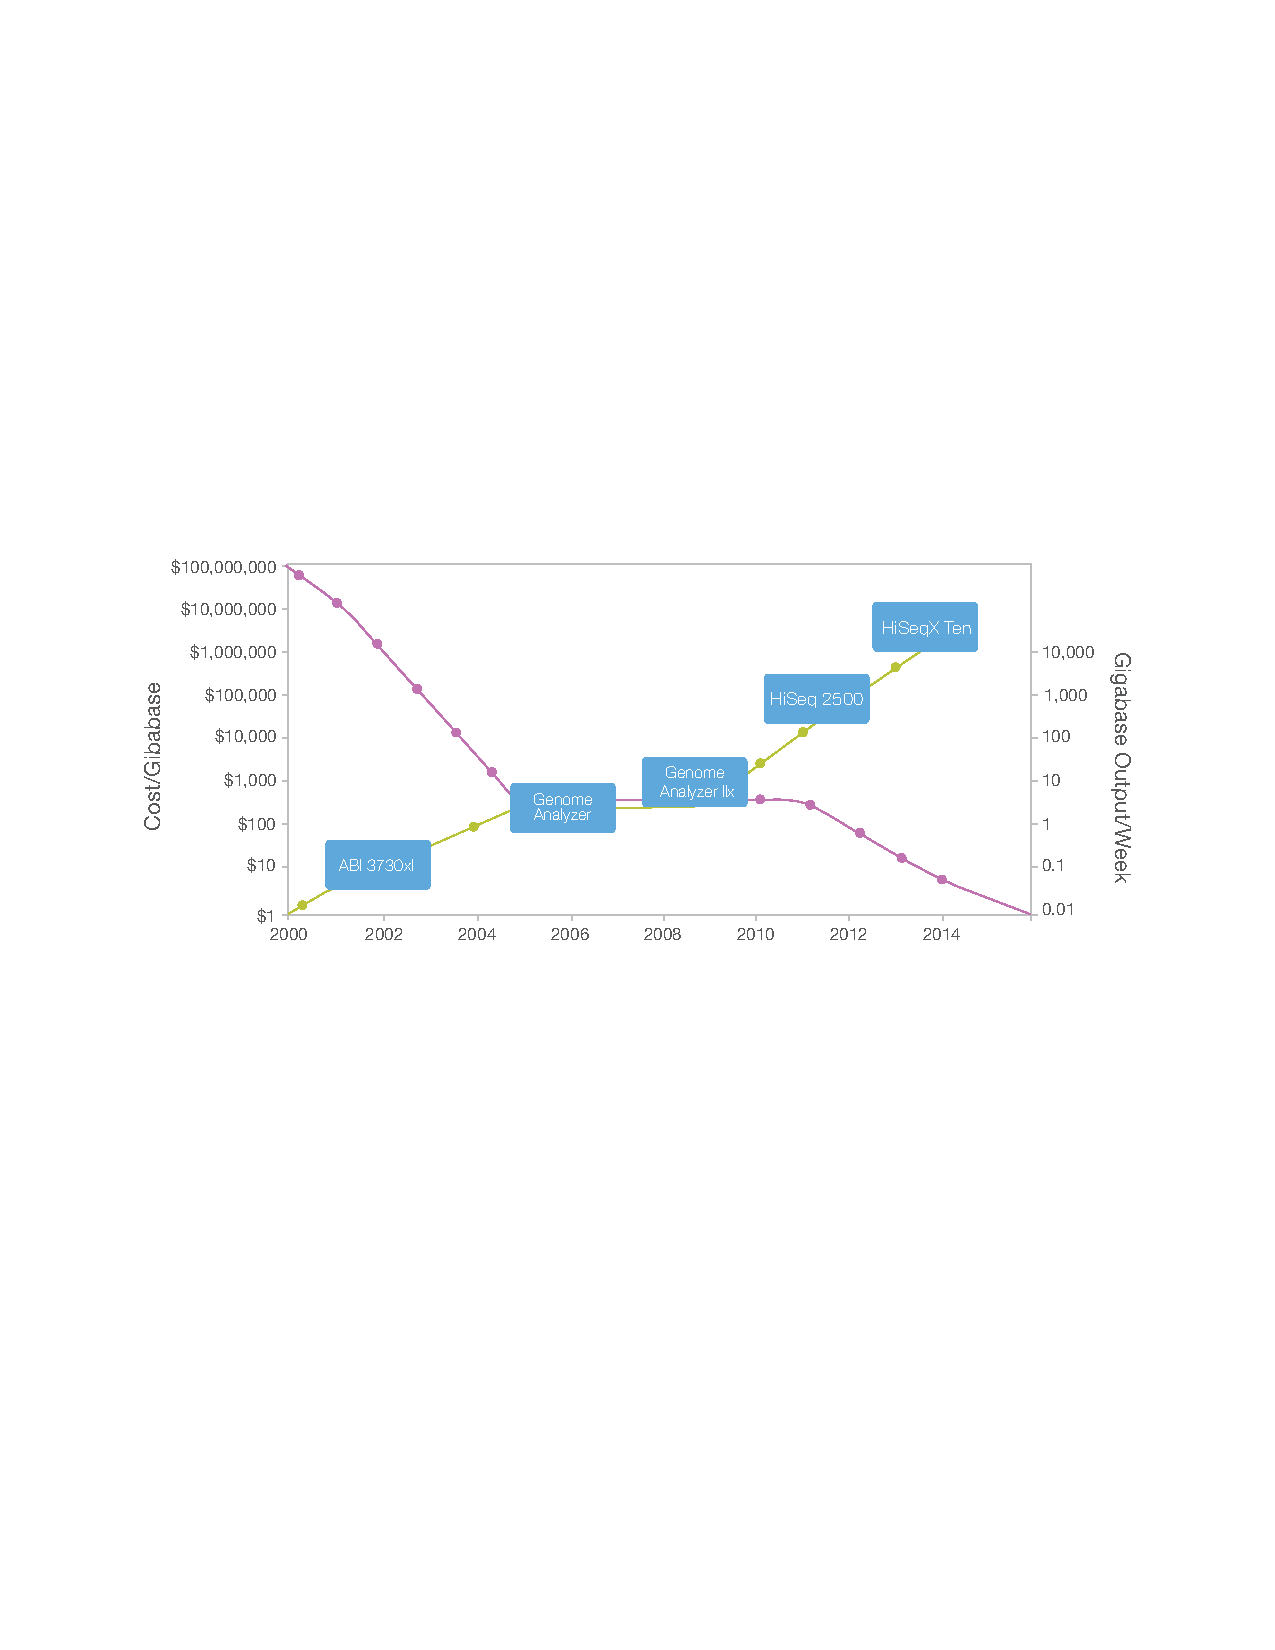
\includegraphics[width = \linewidth]{cost}	
\caption{Cost and Output of DNA sequencing over the from 2000 to 2014}
\end{figure}

\subsection{DNA Sequence Assembly}

Sequence assembly is one of the overarching challenges in bioinformatics.  To understand the assembly problem it helps to understand some basics of DNA sequencing.  Consider a bacterium having a genome comprised of a single 5 megabase (5 million base pairs) chromosome.  Ideally, sequencing machines would start at the beginning of the chromosome and read each of the 5 million base pairs until arriving at the end.  Unfortunately, the current technology is limited to reading sequences between 30 and ~10,000+ bases.  The assembly problem is to take these short segments of DNA called reads and overlap them in such a way to recreate the original 5Mb chromosome.

There are two main classes of assembly algorithms used in de novo assembly:  overlap-layout-consensus (OLC) from \cite{myers2005fragment} and de bruijn graph (DBG) from \cite{zerbino2008velvet} . Similar to the above example, OLC first finds reads with overlapping ends, builds a layout graph based on these overlaps, and lastly generates a consensus sequence as the graph is traversed.  OLC was the first assembly method developed and works well with long-read, low-coverage sequencing technologies like Sanger (and possibly PacBio).

DBG based assemblers convert the set of reads into a set of k-mers (i.e. short DNA sequences of length k).  These k-mers are then used to build a de bruijn graph from which the genomic sequence is inferred.  DBG assemblers work well with high-coverage sequencing methods like Illumina and Ion Torrent.  

\section{Problem formulation}

Throughout the history of the development of genome assembly, there are many formulations of genome assembly from shotgun sequencing data, some of them are more mathematical, while some of them can better represent the practical situations.

Shortest common superstring formulation developed by \cite{kececioglu1995combinatorial} seeks to find the shortest common supersequence for a set of reads. Various maximum-likelihood formulations of the assembly problem proposed by \cite{myers1995toward}, and \cite{medvedev2009maximum} seek to find the sequence that generate the reads with the maximum likelihood. The most widely used formulations, however, are graph based formulations, including de Bruijn Graph by \cite{pevzner2001eulerian}, and String Graph by \cite{myers2005fragment}. 

All the formulations share one common goal: perfect assembly, which means recover the genome perfectly, without any error, from the reads. This does not often happen in real life but is still of theoretical values when assessing different algorithms.


\section{Past}
In this section, I will mainly describe the two mainstreams of genome assembly, DBG and OLC. They are very classic algorithms and is still widely used today. 

\subsection{de Bruijn Graph assembly}

De Bruijn Graph assembly uses a notion called kmer. kmer stands for length-$k$ subsequent string in the reads. The de Bruijn graph assembly pipeline is the following: 
\begin{enumerate}
	\item Get all $k$-mers from all the reads, those are nodes on the graph.
	\item Get all $(k+1)$-mers from all the reads, create edge from $[0:k-1]$ to $[1:k]$.
	\item Merge unambiguous paths, clip dead ends, resolve self loops, etc.
	\item Output contigs. 
\end{enumerate}

Above is the basic idea of de Bruijn Graph assembly, first covered by \cite{pevzner2001eulerian}. Later, there are many variants of such algorithm, mainly on finding different heuristics to deal with different artifacts, resolve repeats, etc. \cite{zerbino2008velvet} developed Velvet, which is still a widely used short read assembler. \cite{peng2010idba} developed IDBA, using a iterative process of construction de Bruijn Graph. \cite{peng2012idba} developed IDBA-UD based on IDBA, and is good at dealing with uneven coverage. \cite{bankevich2012spades} developed spades, it used paired-end information to resolve repeats, which is a highlight. 


\subsection{String Graph assembly}

String graph assembly is first proposed by \cite{myers2005fragment}. The basic process is the following:

\begin{enumerate}
	\item Overlap: create pairwise overlap of all reads
	\item Layout: filter the reads, set a minimum overlap $\theta$, preserve all overlaps exceeding $\theta$, create an edge between these two reads.
	\item Transitive Reduction: reduce transitive edges
	\item Merge nodes, clip dead ends, etc.
	\item Consensus, produce contigs
\end{enumerate}

The overlap step in the String Graph assembly pipeline is the most time consuming, to make this feasible, several improvements are made. \cite{simpson2010efficient} proposed FM-index based method for overlapping. \cite{myers2014efficient} developed Daligner for overlapping. 


An available software using string graph assembly is SGA. 
%\subsection{Comparisons}


\section{Present}
\subsection{Development from theoretical aspects}
Over the years, advances for theory aspects of assembly problem emerge. On core questions is this field is to determine the fundamental limits for genome assembly. The question is what is the coverage required for perfect assembly. However, here we have to make some assumptions: whether the genome is random (for pure theoretical results) or fixed; whether the reads have errors.

\begin{itemize}
	\item Error-free, Random: Fundamental limits for this problem is solved in \cite{motahari2013information}. 
	\item Error-free, Determined: Solved in \cite{bresler2012telescoper}.
	\item Error, Random: Solved in arXiv:1304.2798.
	\item Error, Determined: Solved in arXiv:1501.06194. 
\end{itemize}



\section{Future}
With the emerging technologies at a increasingly rate, we see hope for better genome assembly. Here we show three relatively new technologies and how they became game changers for genome assembly. 

\subsection{SMRT sequencing}
As is shown by \cite{bresler2013optimal}, the bottleneck of genome assembly is the interleaved repeats and triple repeats, if the read length does not exceed $l_{crit}$, perfect assembly is never possible. The widely used Illumina sequencing produces short reads, much shorter than $l_{crit}$, thus perfect assembly from Illumina reads is not quite possible. However, with SMRT reads, which produces long reads, perfect assembly can be addressed. Additionally, Illumina sequencing has severe GC bias, the coverage is uneven, thus creating gaps in the final assembly. SMRT sequencing also could help on this regard. Researchers have already achieved some good assemblies from SMRT data. \cite{chin2013nonhybrid} use a non-hybrid hierarchical approach using Pacbio long reads to generate finished assembly for several bacterial genomes. \cite{loman2015} use nanopore data only to generate finished assembly for several bacterial genomes. Heng Li propose an error-correction free pipeline for SMRT reads, achieving a very short running time. 

\subsection{Barcoding/synthetic long reads}

{\bf GemCode barcoding}

The 10X technology consists of some novel approaches to biological sample preparation, molecular barcoding of the DNA stretches to keep them in tidy little buckets, and software to assemble the DNA in each of those buckets into “linked-reads.” If scientists can consistently get such long, linked reads, they should be able to speed up the sequencing process considerably because they will know more about which parental chromosome the DNA within the “long-read” stretch belongs to.

{\bf Illumina Truseq}

Truseq technology is another technology to use barcodes to maintain long range information while using short read sequencers, it is shown to be useful in work by \cite{McCoy2014}.

\subsection{Contact-map technologies}

Contact-map methods, including Hi-C and 3C, are ways to resolve chromatin structure. Naturally such kind of information could be used for assembly. It is used in scaffolding stage of the assembly, determining orders of contigs. \cite{burton2013chromosome} achieve chromosome scale scaffolding for human genome. It is a way to upgrade existing genomes with Hi-C data. 


\section{Conclusions}

The paper reviews the history and recent development of genome assembly, and points out some key advances in this field. It also gives a discussion about the future of genome assembly.

%\bibliographystyle{natbib}
%\bibliographystyle{achemnat}
%\bibliographystyle{plainnat}
%\bibliographystyle{abbrv}
%\bibliographystyle{bioinformatics}
%
%\bibliographystyle{plain}
%
%\bibliography{Document}

\bibliography{bioinf-sample}

\end{document}
